\documentclass[11pt]{article}
\usepackage[utf8]{inputenc}
\usepackage{listings}
\usepackage{color}
\usepackage{graphicx}
\graphicspath{ {./images/} }
\definecolor{codegreen}{rgb}{0,0.6,0}
\definecolor{codegray}{rgb}{0.5,0.5,0.5}
\definecolor{codepurple}{rgb}{0.58,0,0.82}
\definecolor{backcolour}{rgb}{0.95,0.95,0.92}

%Code listing style named "mystyle"
\lstdefinestyle{mystyle}{
  backgroundcolor=\color{backcolour},   commentstyle=\color{codegreen},
  keywordstyle=\color{magenta},
  numberstyle=\tiny\color{codegray},
  stringstyle=\color{codepurple},
  basicstyle=\footnotesize,
  breakatwhitespace=false,         
  breaklines=true,                 
  captionpos=b,                    
  keepspaces=true,                 
  numbers=left,                    
  numbersep=5pt,                  
  showspaces=false,                
  showstringspaces=false,
  showtabs=false,                  
  tabsize=2
}

%"mystyle" code listing set
\lstset{style=mystyle}
\usepackage{hyperref}
\begin{document}
\title{Detumbling using B-Dot Law}
\date{\ April 2, 2019}
\maketitle

\section{Introduction}
In this paper we try recreating Example 7.5 from the book by Markley and Crassidis for which we write a MATLAB code. To recreate the Example we use Newton's Law of Gravitation for the motion of the satellite and B-Dot Law for Detumbling.

\section{Method}
We first initialize all the values from mentioned Example. Next we run a loop where we start from time $t=0$ and increment $t$ by $dt$ assuming constant acceleration during time interval $dt$. The acceleraton on satellite is due to gravitational force exerted by the Earth. In the loop we use previous known values calculated from pervious iteration to calculate current values. The loop runs till we reach $T$. During the time interval $dt$, we convert ecef coordinates to lattitude, longitude and altitude and find magnetic field at a point using predefined MATLAB functions \href{https://in.mathworks.com/help/aerotbx/ug/ecef2lla.html}{ecef2lla()} and \href{https://in.mathworks.com/help/aerotbx/ug/igrfmagm.html}{igrfmagm()} respectively.
\linebreak\linebreak
Then we apply B-Dot Law such that
$$m=-\frac{k}{||B||} \omega\times b$$
$$L=m\times B$$
where $k$ can be calculated by 
$$k=\frac{4\pi}{T_o_r_b}(1+sin\xi_m)J_m_i_n$$
By Rotational Equations of Motion 
$$L=I\alpha$$
$$\omega_f=\omega_i+\alpha\times dt$$
Now to find next coordinate we use Equations of Motion
$$r_f-r_i=v_i\times dt+\frac{1}{2}a\times dt^2$$
$$v_f=v_i+a\times dt$$
To find acceleration due gravity at $r_f$ towards the center of the Earth
$$a=\frac{GM}{r_f^2}\hat{r_f}=\frac{GM}{r_f^2}\frac{\vec{r_f}}{|r_f|}$$
Now these updated values are used in next iteration for calculating next values and so on.

\section{Code}
\subsection{Initialization}
First we simply initialize or set the intial values $I, r_i, v_i, \omega_i$ and $ \alpha$
\begin{lstlisting}[language=MATLAB]
% The inertia vector of satellite
    inertia = [6400,-76.4,-25.6;-76.4,4730,-40;-25.6,-40,8160]' * 1e-7; % in kg*m^2
% The initial position and velocity of satellite in Earth-Centered Earth-Fixed    
    ini_pos = [1029.7743e3;6699.3469e3;3.7896e3]'; % in m
    ini_vel = [6.2119e3;0.9524e3;4.3946e3]'; % in m/s
% Initial angular velocity and angular acceleration of satellite
    cang = [0.1;0.1;0.1]'; % rad/s
    angacc = [0;0;0]'; % rad/s^2
% Constants
    G = 6.67428e-11; % Earth gravitational constant in m^3/kg*s^2
    M = 5.972e24; % Earth mass in kg
    Re = 6371.2e3; % Radius of earth in m

% Minimum Principal Momentum
    J = 4726.01952; % in kg*m^2
\end{lstlisting}
\subsection{Storing the Output}
We create array initialized to zero to store the output or the answers required to pllot the graph
\begin{lstlisting}[language=MATLAB]
% Final Answers
    ang_vel = zeros(length(t),3); % To store the angular velocity of satellite after dt time
    torque = zeros(length(t),3); % To store the torque of satellite after dt time
\end{lstlisting}
\subsection{Calculated Values}
We calculate required values of different variables
\begin{lstlisting}[language=MATLAB]
%% Calculated Values
% Scalar linear velocity of satellite
    linvel = sqrt(dot(ini_vel, ini_vel)); % in m/s
% The altitude of satellite from earth's surface
    lla = ecef2lla(ini_pos); % ecef2lla() converts ecef coordinates to latitude, longitude and altitude
    alti = lla(3); % in meters
% Distance of satellite from center of earth 
    Rc = Re + alti; % in m
% Time period of satellite
    timePeriod = 2*pi/sqrt(dot(cang, cang)); % in s^-1 Since Time Period = 2pi/(Angular Velocity)
% Accelaration of satellite due to earths gravity
    ini_acc = -ini_pos * (G * M / Rc^2) / sqrt(dot(-ini_pos, -ini_pos)); % in m/s^2 Since acceleration has value of GM/R^2 and in direction opposite to position vector
% Position of satellite after dt time
    ini_pos1 = ini_pos + ini_vel * dt + 0.5 * ini_acc * dt^2; % in m Assuming constant accelaration for dt time Since d = u*t + 0.5*a*t^2
% Angle Of Inclination Of Orbit
    normal = cross(ini_pos, ini_pos1); % Normal to orbit plane
    normalDotK = normal(3) / sqrt(dot(normal, normal)); % Dot product of unit normal vector with k^
    angleOfInclinationOfOrbit = acos(normalDotK); % in rad
% Positive Scalar Gain of Bdot Law
    k = 4*pi*(1 + sin(angleOfInclinationOfOrbit)*J)/timePeriod; % in kg*m^2*s Since k = 4*pi*(1+sin(angle of inclination))*Jmin/Torb

%% Initializations for loop
pos = ini_pos;
vel = ini_vel;
acc = ini_acc;
\end{lstlisting}
\subsection{Main Loop}
Now finally we run the loop for time interval $dt$ such that $t_i=0$ and after each iteration $t_f=t_i+dt$. First we store all the variables in temporary variables for resusing later. Then we use \href{https://in.mathworks.com/help/aerotbx/ug/ecef2lla.html}{ecef2lla()}
to find lattitude, longitude and altitude. Next we use \href{https://in.mathworks.com/help/aerotbx/ug/igrfmagm.html}{igrfmagm()} to find magnetic field $B$ at current position. And now we finally update the values and store them in a 2D array.
\begin{lstlisting}[language=MATLAB]
for i=1:length(t)
     
    veli = vel;
    posi = pos;
    acci = acc;
    cangi = cang;
    
    lla = ecef2lla(posi);
    lat = lla(1); % Latitude
    long = lla(2); % Longitude
    alti = lla(3); % Altitude
    alti = min(alti, 6e5); % Since igrfmagm has a limit on altitude of 6e5
    
    [mag_field_vector1,hor_intensity,declination,inclination,total_intensity] = igrfmagm(alti,lat,long,decyear(2015,7,4),12); % igrfmagm used to calculate the magnetic field of earth at particular position
    mag_field_vector = mag_field_vector1 * 1e-9; % in T Since the function returns the value in nT
    mag_field_vector = mag_field_vector.'; % Taking transpose of the magnetic feild
    
%% B-dot
%   Determinant of Magnetic Field
        detb = sqrt(dot((mag_field_vector),(mag_field_vector)));
%   Magnetic Dipole Moment
        m = ((k)/detb*norm(mag_field_vector))*cross(cang, mag_field_vector); % in A*m^2 Since m = -k (w x b)/||B||
%   Torque
        vtorque = cross(m, mag_field_vector); % in N*m Since T = m x B
%   Angular Accelaration of Satellite
        angacc = vtorque * inv(inertia); % in rad/s^2 Since I x angacc = T
%% Updating loop values

    cang = cangi + (angacc * dt); % calculates the new angular velocity
    pos = posi + (veli * dt) + (0.5 * acci * dt^2); % calculates the new position assuming constant acc for dt time
    vel = veli + (acci * dt); % calculates the new velocity
    acc = -pos * (G * M / Rc^2) / sqrt(dot(pos, pos)); % calculates the new acceleration
% Display the new angular velocity
    disp('new angular velocity');
    disp(cang);
    ang_vel(i,:) = cang;
    torque(i,:) = vtorque;
     
 end
\end{lstlisting}
\subsection{Plots}
We now plot the graphs from obtained values
\begin{lstlisting}[language=MATLAB]
%% Plots
% Plot for Angular velocity
    figure(1)
    subplot(3,1,1)
    plot(t/60,ang_vel(:,1));
    subplot(3,1,2)
    plot(t/60,ang_vel(:,2));
    subplot(3,1,3)
    plot(t/60,ang_vel(:,3));
% Plot for Torque
    figure(2)
    subplot(3,1,1)
    plot(t,torque(:,1));
    subplot(3,1,2)
    plot(t,torque(:,2));
    subplot(3,1,3)
    plot(t,torque(:,3));
\end{lstlisting}
\subsection{Final Code}
\begin{lstlisting}[language=MATLAB]
clear all;
clc;

%% Specify time, where dt is step size and T (in sec) is total time upto which the algorithm will run
dt = 0.30; T = 90*60*3;

t = 0:dt:T;
%% Initializations
% The inertia vector of satellite
    inertia = [6400,-76.4,-25.6;-76.4,4730,-40;-25.6,-40,8160]' * 1e-7; % in kg*m^2
% The initial position and velocity of satellite in Earth-Centered Earth-Fixed    
    ini_pos = [1029.7743e3;6699.3469e3;3.7896e3]'; % in m
    ini_vel = [6.2119e3;0.9524e3;4.3946e3]'; % in m/s
% Initial angular velocity and angular acceleration of satellite
    cang = [0.1;0.1;0.1]'; % rad/s
    angacc = [0;0;0]'; % rad/s^2
% Constants
    G = 6.67428e-11; % Earth gravitational constant in m^3/kg*s^2
    M = 5.972e24; % Earth mass in kg
    Re = 6371.2e3; % Radius of earth in m
% Final Answers
    ang_vel = zeros(length(t),3); % To store the angular velocity of satellite after dt time
    torque = zeros(length(t),3); % To store the torque of satellite after dt time
% Minimum Principal Momentum
    J = 4726.01952; % in kg*m^2

%% Calculated Values
% Scalar linear velocity of satellite
    linvel = sqrt(dot(ini_vel, ini_vel)); % in m/s
% The altitude of satellite from earth's surface
    lla = ecef2lla(ini_pos); % ecef2lla() converts ecef coordinates to latitude, longitude and altitude
    alti = lla(3); % in meters
% Distance of satellite from center of earth 
    Rc = Re + alti; % in m
% Time period of satellite
    timePeriod = 2*pi/sqrt(dot(cang, cang)); % in s^-1 Since Time Period = 2pi/(Angular Velocity)
% Accelaration of satellite due to earths gravity
    ini_acc = -ini_pos * (G * M / Rc^2) / sqrt(dot(-ini_pos, -ini_pos)); % in m/s^2 Since acceleration has value of GM/R^2 and in direction opposite to position vector
% Position of satellite after dt time
    ini_pos1 = ini_pos + ini_vel * dt + 0.5 * ini_acc * dt^2; % in m Assuming constant accelaration for dt time Since d = u*t + 0.5*a*t^2
% Angle Of Inclination Of Orbit
    normal = cross(ini_pos, ini_pos1); % Normal to orbit plane
    normalDotK = normal(3) / sqrt(dot(normal, normal)); % Dot product of unit normal vector with k^
    angleOfInclinationOfOrbit = acos(normalDotK); % in rad
% Positive Scalar Gain of Bdot Law
    k = 4*pi*(1 + sin(angleOfInclinationOfOrbit)*J)/timePeriod; % in kg*m^2*s Since k = 4*pi*(1+sin(angle of inclination))*Jmin/Torb

%% Initializations for loop
pos = ini_pos;
vel = ini_vel;
acc = ini_acc;

%% Main loop
 for i=1:length(t)
     
    veli = vel;
    posi = pos;
    acci = acc;
    cangi = cang;
    
    lla = ecef2lla(posi);
    lat = lla(1); % Latitude
    long = lla(2); % Longitude
    alti = lla(3); % Altitude
    alti = min(alti, 6e5); % Since igrfmagm has a limit on altitude of 6e5
    
    [mag_field_vector1,hor_intensity,declination,inclination,total_intensity] = igrfmagm(alti,lat,long,decyear(2015,7,4),12); % igrfmagm used to calculate the magnetic field of earth at particular position
    mag_field_vector = mag_field_vector1 * 1e-9; % in T Since the function returns the value in nT
    mag_field_vector = mag_field_vector.'; % Taking transpose of the magnetic feild
    
%% B-dot
%   Determinant of Magnetic Field
        detb = sqrt(dot((mag_field_vector),(mag_field_vector)));
%   Magnetic Dipole Moment
        m = ((k)/detb*norm(mag_field_vector))*cross(cang, mag_field_vector); % in A*m^2 Since m = -k (w x b)/||B||
%   Torque
        vtorque = cross(m, mag_field_vector); % in N*m Since T = m x B
%   Angular Accelaration of Satellite
        angacc = vtorque * inv(inertia); % in rad/s^2 Since I x angacc = T
%% Updating loop values

    cang = cangi + (angacc * dt); % calculates the new angular velocity
    pos = posi + (veli * dt) + (0.5 * acci * dt^2); % calculates the new position assuming constant acc for dt time
    vel = veli + (acci * dt); % calculates the new velocity
    acc = -pos * (G * M / Rc^2) / sqrt(dot(pos, pos)); % calculates the new acceleration
% Display the new angular velocity
    disp('new angular velocity');
    disp(cang);
    ang_vel(i,:) = cang;
    torque(i,:) = vtorque;
     
 end

%% Plots
% Plot for Angular velocity
    figure(1)
    subplot(3,1,1)
    plot(t/60,ang_vel(:,1));
    subplot(3,1,2)
    plot(t/60,ang_vel(:,2));
    subplot(3,1,3)
    plot(t/60,ang_vel(:,3));
% Plot for Torque
    figure(2)
    subplot(3,1,1)
    plot(t,torque(:,1));
    subplot(3,1,2)
    plot(t,torque(:,2));
    subplot(3,1,3)
    plot(t,torque(:,3));

\end{lstlisting}
\section{Results}
Below are the plots of $\omega_1,\omega_2$ and $\omega_3$ in Figure 1 and plots of $L_1,L_2$ and $L_3$ in Figure 2
\linebreak
\includegraphics[scale=0.37]{Angular_Velocity.jpg}
\begin{center}
    Figure 1
\end{center}
\linebreak
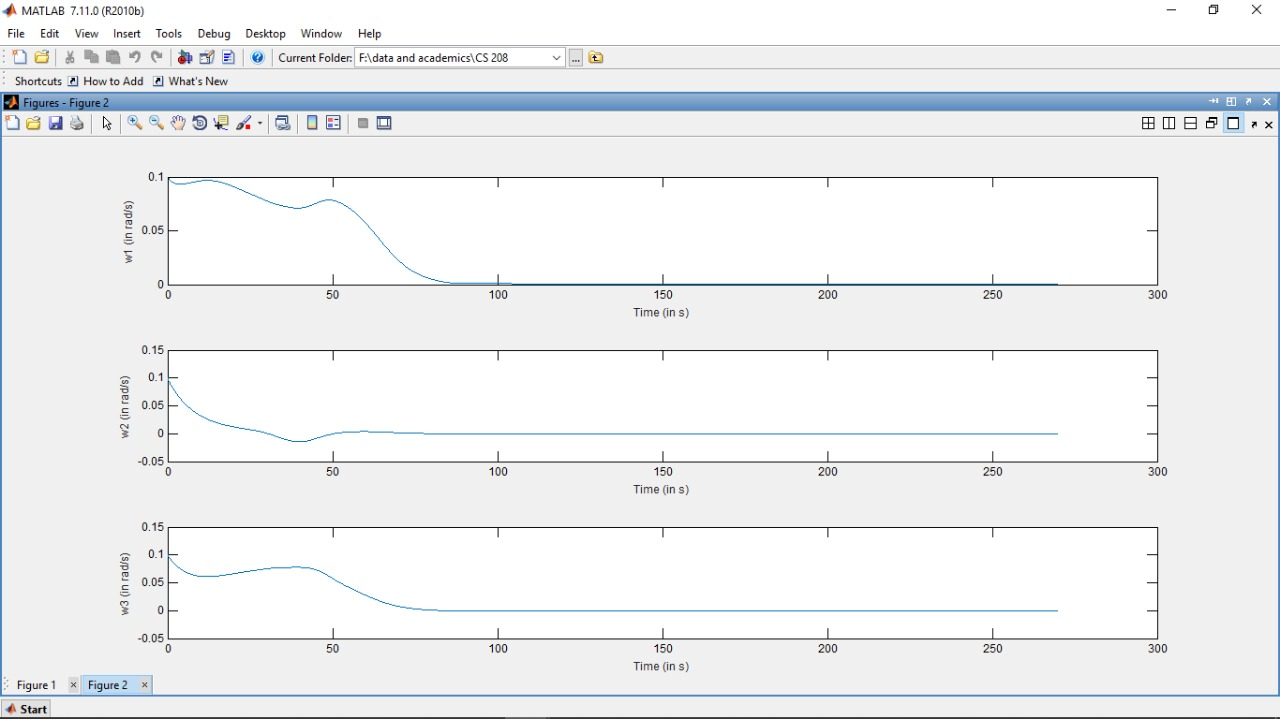
\includegraphics[scale=0.37]{Torque.jpg}
\begin{center}
    Figure 2
\end{center}
\end{document}
